\chapter{Control potencia - frecuencia.}
\section{Esquema del control de un generador síncrono.}
En el tema 7 se estudio el control Q-V. En este tema se estudiará el control P-f.
\begin{figure}[H]
	\centering
	\begin{circuitikz}
		\tikzstyle{every node}=[font=\normalsize]
		\draw [short] (7.25,10.25) -- (7.25,8.75);
		\draw [short] (6.25,9.25) -- (7.25,8.75);
		\draw [short] (6.25,9.75) -- (7.25,10.25);
		\node [font=\normalsize] at (3.5,10.75) {};
		\node [font=\normalsize] at (6.75,9.5) {TV};
		\draw [short] (7.25,9.75) -- (9,9.75);
		\draw [short] (7.25,9.25) -- (9,9.25);
		\draw [short] (9.75,10) -- (10,10);
		\draw [short] (10,10) -- (10,9.75);
		\draw [short] (9.75,9) -- (10,9);
		\draw [short] (10,9) -- (10,9.25);
		\draw [short] (10,9.25) -- (11.8,9.25);
		\draw [short] (10,9.75) .. controls (12.5,9.75) and (10.25,9.75) .. (11.8,9.75);
		\draw  (12.5,9.5) circle (0.75cm) node {\normalsize G} ;
		\draw [line width=0.2pt, short] (12.25,9.25) .. controls (12.5,9.5) and (12.5,9) .. (12.75,9.25);
		\draw [short] (13.25,9.5) -- (15.5,9.5);
		\draw [short] (14.75,9.5) -- (14.75,7);
		\draw  (11.5,7.5) rectangle (13.5,6.5);
		\node [font=\normalsize] at (12.5,7.25) {Regulador};
		\node [font=\normalsize] at (12.5,6.75) {AVR};
		\draw (11.75,8.25) to[L ] (13.25,8.25);
		\draw [short] (11.75,8.25) -- (11.75,7.5);
		\draw [short] (13.25,8.25) -- (13.25,7.5);
		\draw [line width=0.2pt, short] (13.5,9.25) -- (13.75,9.75);
		\draw [line width=0.2pt, short] (13.75,9.25) -- (14,9.75);
		\draw [line width=0.2pt, short] (14,9.25) -- (14.25,9.75);
		\draw [line width=0.2pt, short] (14.25,9.25) -- (14.5,9.75);
		\draw [short] (9.75,10) -- (9.75,11.25);
		\draw [short] (9.75,10) -- (9.5,10);
		\draw [short] (9.5,10) -- (9.5,9.75);
		\draw [short] (9.5,9.25) -- (9.5,9);
		\draw [short] (9.5,9) -- (9.75,9);
		\draw [short] (9,9.75) -- (9.5,9.75);
		\draw [short] (9,9.25) -- (9.5,9.25);
		\draw [short] (6.25,9.75) -- (6.25,9.25);
		\draw  (8.75,12.25) rectangle (10.75,11.25);
		\node [font=\normalsize] at (9.75,12) {Regulador};
		\node [font=\normalsize] at (9.75,11.5) {velocidad};
		\draw [->, >=Stealth] (8,10) .. controls (8.25,9.5) and (8.25,9.5) .. (8,9) ;
		\draw [->, >=Stealth] (8.75,10) .. controls (9,9.5) and (9,9.5) .. (8.75,9) ;
		\draw [->, >=Stealth] (11.25,9) .. controls (11,9.5) and (11,9.5) .. (11.25,10) ;
		\node [font=\normalsize] at (8,8.75) {n};
		\node [font=\normalsize] at (10,10.75) {n};
		\node [font=\normalsize] at (11.25,10.25) {$T_{elec}$};
		\node [font=\normalsize] at (8.75,8.75) {$T_{mec}$};
		\draw [->, >=Stealth] (9.75,10) -- (9.75,11.25);
		\draw [->, >=Stealth] (12,11.75) -- (10.75,11.75);
		\draw [->, >=Stealth] (12.5,5.75) -- (12.5,6.5);
		\draw [->, >=Stealth] (11.5,7.75) -- (11.5,8.25);
		\draw [->, >=Stealth] (14.75,7) -- (13.5,7);
		\node [font=\normalsize] at (14.75,8.25) {};
		\node [font=\normalsize] at (12.5,5.5) {$V_{ref}$};
		\node [font=\normalsize] at (11.25,8) {$I_{ex}$};
		\node [font=\normalsize] at (15,8) {V};
		\node [font=\normalsize] at (12.5,11.75) {$P_{ref}$};
		\draw  (8,11.75) circle (0.5cm);
		\draw [short] (8.75,11.75) -- (8.5,11.75);
		\node [font=\normalsize] at (8,11.75) {$M$};
		\draw [short] (7.5,11.75) -- (5.75,11.75);
		\draw [->, >=Stealth] (5.75,11.75) -- (5.75,11.25);
		\draw [short] (5.75,11.25) -- (6.25,11.5);
		\draw [short] (5.75,11.25) -- (6.25,11);
		\draw [short] (6.25,11) -- (6.25,11.5);
		\draw [short] (5.75,11.25) -- (5.25,11.5);
		\draw [short] (5.25,11.5) -- (5.25,11);
		\draw [short] (5.25,11) -- (5.75,11.25);
		\draw [short] (6.75,10) -- (6.75,11.25);
		\draw [short] (6.25,11.25) -- (6.75,11.25);
		\draw [short] (5.25,11.25) -- (4.75,11.25);
		\node [font=\normalsize] at (8,12.5) {$Servomotor$};
		\node [font=\normalsize] at (4,11.5) {$Entrada$};
		\node [font=\normalsize] at (4,11) {$vapor$};
		\draw [ color={rgb,255:red,2; green,141; blue,37} , dashed] (10.5,10.75) rectangle  (16,5);
		\draw [ color={rgb,255:red,234; green,72; blue,72}, dashed] (13,10.75) -- (13,13.5);
		\draw [ color={rgb,255:red,234; green,72; blue,72}, dashed] (13,13.5) -- (3.25,13.5);
		\draw [ color={rgb,255:red,234; green,72; blue,72}, dashed] (3.25,13.5) -- (3.25,7.75);
		\draw [ color={rgb,255:red,234; green,72; blue,72}, dashed] (3.25,7.75) -- (10.5,7.75);
		\node [font=\normalsize, color={rgb,255:red,234; green,72; blue,72}] at (4.25,13) {Control P-f};
		\node [font=\normalsize, color={rgb,255:red,62; green,167; blue,89}] at (14.75,5.5) {Control Q-V};
	\end{circuitikz}
	\label{fig:my_label}
\end{figure}
\section{Control potencia - frecuencia desde el punto de vista del mercado de servicios complementarios.}
Repasando el tema 4, el control se divide en primario, secundario y terciario.
\subsection{Control primario.}
Es una respuesta a nivel de central con un tiempo de actuación de 2 a 20 segundos.
\begin{itemize}
	\item [-] Es un servicio obligatorio no retribuido.
	\item [-] Su objetivo es mantener la estabilidad de la frecuencia del sistema de forma automática.
	\item [-] Los reguladores de velocidad actúan de manera automática para corregir desequilibrios de variación de carga de hasta el 1.5\% de la potencia nominal.
	\begin{itemize}
		\item En 15s desvíos de frecuencia $\le 100mHz$.
		\item Lineal entre 15 y 30s antes desvíos entre $100$ y $200mHz$.
	\end{itemize}
\end{itemize}
\subsection{Control secundario.}
Es una respuesta para corregir efectos no resueltos por la regulación primaria con un tiempo de respuesta entre 20 segundos y 2 minutos:
\begin{itemize}
	\item [-] Desviación de la frecuencia respecto a la de referencia.  
	\item [-] El reparto de demando queda determinada por el estatismo del generador (se verá más adelante) y no se cumplen los flujos de potencia programados.
\end{itemize}
La regulación secundaria es un servicio voluntario y retribuido. 
\subsection{Control terciario.}
Es el encargado de establecer la consigna de producción base de potencia para cada generador para restablecer la reserva de regulación rodante. El tiempo de respuesta es de 10 a 15 minutos. La reserva es determinada por el operador del sistema, REE, para los generadores habilitados. La reserva a subir se establece entre el 40\% y el 100\%.


\section{Dinámica del rotor}
\begin{figure}[H]
	\begin{minipage}{0.5\textwidth}
		\begin{figure}[H]
			\centering
			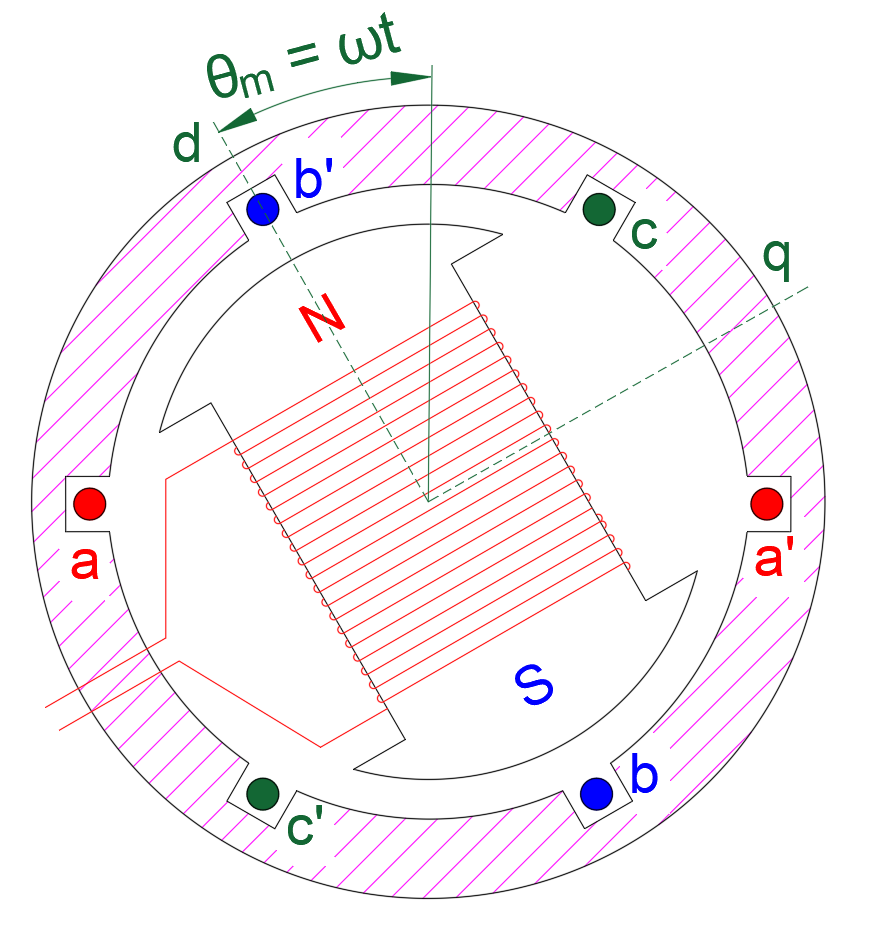
\includegraphics[width=0.7\linewidth]{res/tema6/ejes_dq}
			\label{fig:ejesdq}
		\end{figure}
	\end{minipage}
	\begin{minipage}{0.5\textwidth}
	La ecuación que gobierna la dinámica del rotor de un generador síncrono es:
	\[J\frac{d^2\theta_m}{dt^2}=T_{mec}-T_{elec}\]
	\[J=\frac{1}{2}mr^2\]
	Donde:
	\begin{itemize}
		\item [-] \textbf{J}: momento de inercia $\left[kg \cdot m^2\right]$.
		\item [-] \textbf{$\mathbf{\theta_m}$}: desplazamiento angular del rotor $[rad]$.
		\item [-] \textbf{$\mathbf{T_{mec}}$}: par mecánico $[kg \cdot N]$. Depende del caudal.
		\item [-] \textbf{$\mathbf{T_{elec}}$}: par eléctrico $[kg \cdot N]$. Depende de la potencia demandada.
	\end{itemize}
	\end{minipage}
\end{figure}
En régimen permanente el par eléctrico es igual al mecánico y por tanto la velocidad, n, es constante.
\[\frac{d^2\theta_m}{dt^2}=0 \rightarrow n=cte\]
\begin{itemize}
	\item [-] Si $T_{mec} > T_{elec}$ el eje se acelera.
	\item [-]  Si $T_{mec} < T_{elec}$ el eje se ralentiza.
\end{itemize}




Desarrollando:
\[J\frac{d^2\theta_m}{dt^2}=T_{mec}-T_{elec}\]
\[
\theta_m = \underbrace{\omega_s}_{\text{cte}} t + \delta_m
\]
\[J\frac{d^2\theta_m}{dt^2}=J\frac{d^2\delta_m}{dt^2}=J\frac{d^2\Delta \omega_r}{dt^2}\]




Donde:
\begin{itemize}
	\item [-] $ \omega_s$ es la velocidad síncrona.
	\item [-] $\delta_m $ es el desplazamiento angular del rotor (diagrama de máquina síncrona).
\end{itemize}
\newpage
Tomando como valores base:
\begin{itemize}
	\item [-] $S_B=S_N [MVA]$
	\item [-] $\omega_B=\omega_S \left[\frac{rad}{s}\right]$
	\item [-] $T_B=\frac{S_B}{\omega_B} [N\cdot m]$
\end{itemize}



Operando:
\[J\frac{d^2\Delta \omega_r}{dt^2}=T_{mec}-T_{elec}
\rightarrow 
\frac{\frac{d\Delta \omega_r}{dt}}{\omega_B}=\frac{1}{J}\left(\Delta T_{mec}-\Delta T_{elec}\right)\cdot \left(\frac{S_B}{T_B \cdot \omega_B^2}\right)\]
\[\frac{d\Delta \omega_{r_{p.u.}}}{dt}=
\frac{1}{2H}\left(\Delta T_{mec_{p.u.}}-\Delta T_{elec_{p.u.}}\right)\]





El coeficiente H es la constante de inercia normalizada y se define como:
\[H=\frac{\text{Energía cinética almacenada}}{\text{Potencia aparante nominal}}=\frac{J \omega_B^2}{2S_B} \left[\frac{MJ}{MVA}\right] o [s]\]

Además, a partir de la expresión se puede deducir que:
\begin{itemize}
	\item [-] Si la potencia (P) sube, la frecuencia (f) baja.
	\item [-] Si la potencia (P) baja, la frecuencia (f) sube.
\end{itemize}



Pasando al dominio de Laplace:
\[s\Delta \omega_{r}(s)=\frac{1}{2H}\left[\Delta T_{mec}(s)-\Delta T_{elec}(s)\right]\]
\begin{figure}[H]
	\centering
		\begin{circuitikz}
			\tikzstyle{every node}=[font=\normalsize]
			\draw  (5,11.5) circle (0.75cm);
			\node [font=\normalsize] at (4,11.75) {+};
			\node [font=\normalsize] at (5.25,10.5) {-};
			\draw [->, >=Stealth] (5,9.25) -- (5,10.75);
			\draw [->, >=Stealth] (3.25,11.5) -- (4.25,11.5);
			\node [font=\normalsize] at (3,12) {$\Delta P_{mec} (s)$};
			\node [font=\normalsize] at (5,9) {$\Delta P_{elec} (s)$};
			\draw  (7.5,12.25) rectangle  node {\normalsize $\frac{1}{2Hs}$} (11,11);
			\draw [->, >=Stealth] (5.75,11.5) -- (7.5,11.5);
			\draw [->, >=Stealth] (11,11.5) -- (13.25,11.5);
			\node [font=\normalsize] at (13.5,12) {$\Delta \omega_r (s)$};
		\end{circuitikz}
	\label{fig:my_label}
\end{figure}
\subsection{Valores de la constante de inercia.}
\begin{table}[H]
	\centering
	\renewcommand{\arraystretch}{1.5}
	\begin{tabular}{ccc}
		\hline
		&Velocidad de síncronismo& H\\
		\hline
		Turbogenerador & 3000 rpm&6-9 $\frac{MJ}{MVA}$ \\
		\hline
		Generador hidráulico & $<$200 rpm&2-3 $\frac{MJ}{MVA}$ \\
		\hline
		Generador hidráulico & $>$200 rpm&2-4 $\frac{MJ}{MVA}$ \\
		\hline
	\end{tabular}
\end{table}
\section{Respuesta de la demanda ante una desviación de la frecuencia.}
En función del tipo de carga la desviación de la frecuencia afecta de manera distinta al sistema.
\begin{itemize}
	\item [-] Cargas resistivas: $P=RI^2$ $\rightarrow$ No les influye un $\Delta f$.
	\item [-] Cargas inductivas: la frecuencia modifica el comportamiento:
	\begin{itemize}
		\item Si $f\uparrow$ aumentan las pérdidas $\Delta P_D \uparrow$.
		\item  Si $f\downarrow$ disminuyen las pérdidas $\Delta P_D \downarrow$.
		\item La frecuencia modifica la velocidad de giro.
	\end{itemize}
\end{itemize}



Aún así, la respuesta del incremento de potencia $\Delta P_D$ es subamortiguada.
 \[\Delta P_{D_{inicial}}\ne \Delta P_{D_{final}}\] 
  
  Por tanto, se linealiza.
\[\Delta P_{D_f}=\Delta P_{D_{inicial}}+\frac{\partial P_D}{\partial f}\Delta f\]
\[\frac{\partial P_D}{\partial f}=\frac{1}{tg(\gamma)}=D\]
\begin{figure}[H]
	\centering
		\begin{circuitikz}
			\tikzstyle{every node}=[font=\normalsize]
			\draw [->, >=Stealth] (6,7.5) -- (6,13.75);
			\draw [->, >=Stealth] (5.5,8) -- (12,8);
			\node [font=\normalsize] at (13,8) {$P_D (MW)$};
			\node [font=\normalsize] at (6,14) {$f(HZ)$};
			\node [font=\normalsize] at (8.5,7.25) {$P_{D0}$};
			\node [font=\normalsize] at (5,11.5) {$f_0 = 50Hz$};
			\node [font=\normalsize] at (10.5,12.75) {$\gamma$};
			\draw [dashed] (6,10.75) -- (7.75,10.75);
			\draw [dashed] (7.75,10.75) -- (7.75,8);
			\draw [dashed] (8.5,8) -- (8.5,11.5);
			\draw [dashed] (6,11.5) -- (8.5,11.5);
			\draw [dashed] (6,12.25) -- (9.25,12.25);
			\draw [dashed] (9.25,12.25) -- (9.25,8);
			\draw [short] (7.25,10.25) -- (8.5,11.5);
			\draw [short] (8.5,11.5) -- (10.25,13.25);
			\draw [dashed] (9.25,12.25) -- (10.75,12.25);
			\draw [<->, >=Stealth] (10,13) .. controls (10.25,12.5) and (10.25,12.5) .. (10.25,12.25);
		\end{circuitikz}
	\label{fig:my_label}
\end{figure}

La variable D, es la característica de respuesta en frecuencia de la demanda.
\[D \left[\frac{MW}{Hz}\right]\]




Incluyendo la demanda en el diagrama de bloques:
\begin{figure}[!ht]
	\centering
		\begin{circuitikz}
			\tikzstyle{every node}=[font=\normalsize]
			\draw  (5.75,10.5) circle (0.75cm);
			\draw [->, >=Stealth] (6.5,10.5) -- (8.25,10.5);
			\draw  (8.25,10) rectangle  node {\normalsize $\frac{1}{2Hs+D}$} (11.25,11);
			\draw [->, >=Stealth] (11.25,10.5) -- (12.75,10.5);
			\node [font=\normalsize] at (13.25,10.5) {$\Delta\omega_r$};
			\node [font=\normalsize] at (4.75,11) {+};
			\node [font=\normalsize] at (6.25,9.5) {-};
			\draw [->, >=Stealth] (5.75,8.25) -- (5.75,9.75);
			\draw [->, >=Stealth] (3.5,10.5) -- (5,10.5);
			\node [font=\normalsize] at (2.75,10.5) {$\Delta P_{mec}(s)$};
			\node [font=\normalsize] at (5.75,8) {$\Delta P_{elec}(s) =\Delta P_D (s)$};
		\end{circuitikz}
	\label{fig:my_label}
\end{figure}

Por tanto, la ecuación del incremento de frecuencia queda como:
\[\Delta \omega_{r}(s)=\frac{1}{2Hs+D}\left[\Delta T_{mec}(s)-\Delta T_{elec}(s)\right]\]
\newpage
\section{Regulador de velocidad.}
Tiene como objetivo mandar al servomotor abrir o cerrar la válvula que regula el caudal para aumentar la potencia mecánica en el eje.
\subsection{Regulador astático.}
Solo se emplea para generadores aislados de la red y se corrige la frecuencia a 50Hz mediante variación de potencia mecánica.
\subsection{Regulador con estatismo positivo.}
Se emplea para generadores no aislados de la red. Este regulador permite que f quede desviada en unos margenes de tolerancia ($\Delta f_{max} = \pm 0,25 Hz$) y se regula mediante generadores en paralelo hasta la plena carga (pc). 
\begin{figure}[H]
	\centering
		\begin{circuitikz}
			\tikzstyle{every node}=[font=\normalsize]
			\draw [->, >=Stealth] (4.75,10) -- (4.75,14.25);
			\draw [->, >=Stealth] (4.5,10.5) -- (9,10.5);
			\node [font=\normalsize] at (9.25,10.5) {$P_D$};
			\node [font=\normalsize] at (4.75,14.5) {$\omega$};
			\node [font=\normalsize] at (4.5,12.75) {$\omega_s$};
			\node [font=\normalsize] at (4.5,12) {$\omega_{pc}$};
			\draw [dashed] (4.75,12) -- (6.75,12);
			\draw [dashed] (4.75,12.75) -- (9.75,12.75);
			\draw [short] (6.75,12) -- (4.75,14);
			\node [font=\normalsize] at (5,13.1) {$\alpha$};
			\draw [short] (6,12.75) -- (9.75,14);
			\draw [short] (6,12.75) -- (5.25,12.5);
			\node [font=\normalsize] at (8,13.05) {$\gamma$};
			\draw [<->, >=Stealth] (7.5,13.25) .. controls (7.75,13) and (7.75,13) .. (7.75,12.75);
			\draw [<->, >=Stealth] (5.25,12.75) .. controls (5.25,13) and (5.25,13) .. (5.5,13.25);
			\draw [dashed] (6,12.75) -- (6,10.5);
			\node [font=\normalsize] at (6,10.25) {$P_{fin}$};
			\node [font=\normalsize] at (10.25,14.25) {Respuesta de la demanda};
			\node [font=\normalsize] at (6,14.25) {Regulador};
			\draw [->, >=Stealth, dashed] (6,14) -- (5.25,13.5);
		\end{circuitikz}	
	\label{fig:my_label}
\end{figure}
Traduciéndolo en ecuaciones:
\[\Delta P_m=\Delta P_{elec}=-k\Delta \omega \rightarrow k=-\frac{\Delta P_{elec}}{\omega} \rightarrow tg(\alpha)=\frac{1}{K}=R\]
\[\Delta \omega=\omega_0 -\Delta_{pc}\]

Donde R es la constante de estatismo del generador.
\[R \left[\frac{Hz}{MW}\right]\]

Cada generador tiene un valor de R diferente y ante un incremento de potencia demandada, esta, se reparte de manera proporcional a la R de cada generador. Por tanto, el diagrama de bloques:
\begin{figure}[H]
	\centering
		\begin{circuitikz}
			\tikzstyle{every node}=[font=\normalsize]
			\draw  (5.75,10.5) circle (0.75cm);
			\draw [->, >=Stealth] (6.5,10.5) -- (8.25,10.5);
			\draw  (8.25,10) rectangle  node {\normalsize $\frac{1}{2Hs+D}$} (11.25,11);
			\draw [->, >=Stealth] (11.25,10.5) -- (12.75,10.5);
			\node [font=\normalsize] at (13.25,10.5) {$\Delta\omega_r$};
			\node [font=\normalsize] at (4.75,11) {+};
			\node [font=\normalsize] at (6.25,9.5) {-};
			\draw [->, >=Stealth] (5.75,8.25) -- (5.75,9.75);
			\draw [->, >=Stealth] (3.5,10.5) -- (5,10.5);
			\node [font=\normalsize] at (5.75,8) {$\Delta P_{elec}(s) =\Delta P_D (s)$};
			\draw  (3,11) rectangle  node {\normalsize $-\frac{1}{R}$} (4,12);
			\draw [short] (3.5,10.5) -- (3.5,11);
			\draw [short] (12,10.5) -- (12,12.5);
			\draw [short] (12,12.5) -- (3.5,12.5);
			\draw [->, >=Stealth] (3.5,12.5) -- (3.5,12);
		\end{circuitikz}
	\label{fig:my_label}
\end{figure}
La nueva relación entre demanda y velocidad angular queda como:
\[\Delta \omega_r(s)=\frac{-\Delta P_D(s)}{2Hs+D+\frac{1}{R}}=\frac{-\Delta P_D(s)}{2Hs+\beta}\]


Donde $\beta$ es la característica de la respuesta en frecuencia del sistema.
\[\beta \left[\frac{MW}{Hz}\right]\]

\section{Participación en la regulación de generadores en paralelo.}
Se tienen 2 generadores en paralelo donde cada uno tiene su potencia $S_N$ y estatismo R.
\begin{figure}[H]
	\centering
		\begin{circuitikz}
			\tikzstyle{every node}=[font=\normalsize]
			\draw  (2.75,11.75) circle (0.75cm) node {\normalsize $G_1$} ;
			\draw  (6.25,11.75) circle (0.75cm) node {\normalsize $G_2$} ;
			\draw [short] (2,9.75) -- (7,9.75);
			\draw [short] (2.75,11) -- (2.75,9.75);
			\draw [short] (6.25,11) -- (6.25,9.75);
			\draw [short] (4.75,9.75) -- (4.75,8.5);
			\draw [->, >=Stealth] (4.75,9.75) -- (4.75,9);
			\draw [->, >=Stealth] (6.25,11) -- (6.25,10.25);
			\draw [->, >=Stealth] (2.75,11) -- (2.75,10.25);
			\node [font=\normalsize] at (3.25,10.5) {$P_{g1}$};
			\node [font=\normalsize] at (6.25,9) {$P_D=P_{g1}+P_{g2}$};
			\node [font=\normalsize] at (6.75,10.5) {$P_{g2}$};
		\end{circuitikz}
	\label{fig:my_label}
\end{figure}


Ante un aumento de la demanda disminuye la frecuencia.
\begin{figure}[H]
	\centering
		\begin{circuitikz}
			\tikzstyle{every node}=[font=\normalsize]
			\draw [->, >=Stealth] (3,10.5) -- (3,15.25);
			\draw [->, >=Stealth] (2.5,10.75) -- (12.25,10.75);
			\draw [ color={rgb,255:red,255; green,0; blue,0}, short] (3,14.25) -- (6.75,13.5);
			\draw [ color={rgb,255:red,0; green,85; blue,255}, short] (3,15) -- (6.75,13.5);
			\draw [ color={rgb,255:red,253; green,30; blue,30}, short] (6.75,13.5) -- (11.25,12.75);
			\draw [ color={rgb,255:red,0; green,85; blue,255}, short] (6.75,13.5) -- (10.5,12.25);
			\draw [dashed] (3,14) -- (5.5,14);
			\draw [dashed] (6.75,13.5) -- (3,13.5);
			\draw [dashed] (4.25,14) -- (4.25,9.75);
			\draw [ color={rgb,255:red,0; green,85; blue,255}, dashed] (5.5,14) -- (5.5,10.25);
			\draw [ color={rgb,255:red,255; green,0; blue,0}, dashed] (6.75,13.5) -- (6.75,9.75);
			\draw [ color={rgb,255:red,0; green,85; blue,255}, <->, >=Stealth] (5.5,10.25) -- (6.75,10.25)node[pos=0.5, fill=white]{$\Delta  P_{g1}$};
			\draw [ color={rgb,255:red,255; green,0; blue,0}, <->, >=Stealth] (4.25,9.75) -- (6.75,9.75)node[pos=0.5, fill=white]{$\Delta  P_{g2}$};
			\node [font=\normalsize] at (12.5,10.75) {$P_D$};
			\node [font=\normalsize] at (3,15.5) {$\omega$};
			\node [font=\normalsize] at (2.5,14) {$\omega_0$};
			\node [font=\normalsize] at (2.5,13.5) {$\omega_f$};
			\node [font=\normalsize, color={rgb,255:red,253; green,30; blue,30}] at (11.5,12.75) {$G_2$};
			\node [font=\normalsize, color={rgb,255:red,0; green,85; blue,255}] at (10.75,12.25) {$G_1$};
		\end{circuitikz}
	\label{fig:my_label}
\end{figure}

Donde el generador con menor estatismo proporcionará un mayor incremento de potencia demandada.
\[\Delta P_{D_t}=\Delta P_D +D\Delta f\]
\[\Delta P_{g_1}+\Delta P_{g_2}=\Delta P_D +D\Delta f\]
\[-\frac{\Delta f}{R_1}-\frac{\Delta f}{R_2}=\Delta P_D +D\Delta f\]
\[\Delta f\left(D+\frac{1}{R_1}+\frac{1}{R_2}\right)=-\Delta P_D\]
\[\Delta f=-\frac{\Delta P_D}{D+\frac{1}{R_1}+\frac{1}{R_2}}=-\frac{\Delta P_D}{\beta}\]
\section{Participación de distintas áreas en la regulación.}
\begin{figure}[H]
	\centering
		\begin{circuitikz}
			\tikzstyle{every node}=[font=\normalsize]
			\draw  (2.25,14.75) circle (0.5cm) node {\normalsize $G_1$} ;
			\draw  (3.75,13.25) circle (0.5cm) node {\normalsize $G_4$} ;
			\draw  (2.25,11.75) circle (0.5cm) node {\normalsize $G_3$} ;
			\draw  (0.75,13.25) circle (0.5cm) node {\normalsize $G_2$} ;
			\draw [short] (1.75,14) -- (2.75,14);
			\draw [short] (3,13.75) -- (3,12.75);
			\draw [short] (1.75,12.5) -- (2.75,12.5);
			\draw [short] (1.5,12.75) -- (1.5,13.75);
			\draw [short] (1.25,13.25) -- (1.5,13.25);
			\draw [short] (2.25,14.25) -- (2.25,14);
			\draw [short] (3,13.25) -- (3.25,13.25);
			\draw [short] (2.25,12.25) -- (2.25,12.5);
			\draw [short] (1.5,13.5) -- (2,13.5);
			\draw [short] (2,13.5) -- (2,14);
			\draw [short] (1.5,13) -- (2,13);
			\draw [short] (2,13) -- (2,12.5);
			\draw [short] (2.5,12.5) -- (2.5,13);
			\draw [short] (2.5,13) -- (3,13);
			\draw [short] (2.5,14) -- (2.5,13.5);
			\draw [short] (2.5,13.5) -- (3,13.5);
			\draw [short] (3,12.75) -- (3.25,12.75);
			\draw [->, >=Stealth] (3.25,12.75) -- (3.25,12);
			\node [font=\normalsize] at (8.75,14.75) {$G_1$};
			\draw  (8.75,14.75) circle (0.5cm) node {\normalsize $G_1$} ;
			\node [font=\normalsize] at (8.75,14) {};
			\node [font=\normalsize] at (8.75,14) {};
			\node [font=\normalsize] at (9,13.75) {};
			\draw [short] (8.25,14) -- (9.25,14);
			\node [font=\normalsize] at (9.25,13.5) {};
			\draw [short] (9.5,13.75) -- (9.5,12.75);
			\draw  (10.25,13.25) circle (0.5cm) node {\normalsize $G_4$} ;
			\node [font=\normalsize] at (9.5,13.25) {};
			\node [font=\normalsize] at (9.5,12.75) {};
			\draw [->, >=Stealth] (9.75,12.75) -- (9.75,12);
			\draw  (8.75,11.75) circle (0.5cm) node {\normalsize $G_3$} ;
			\node [font=\normalsize] at (8.75,12.25) {};
			\draw [short] (8.25,12.5) -- (9.25,12.5);
			\node [font=\normalsize] at (9,12.75) {};
			\node [font=\normalsize] at (9.25,13) {};
			\draw [short] (8.5,13) -- (8.5,12.5);
			\node [font=\normalsize] at (8.25,13) {};
			\draw [short] (8,12.75) -- (8,13.75);
			\draw [short] (8,13.5) -- (8.5,13.5);
			\node [font=\normalsize] at (8.5,13.75) {};
			\node [font=\normalsize] at (7.75,13.25) {};
			\draw  (7.25,13.25) circle (0.5cm) node {\normalsize $G_2$} ;
			\draw [short] (8,13) -- (8.5,13);
			\draw [short] (8.5,13.5) -- (8.5,14);
			\draw [short] (9,14) -- (9,13.5);
			\draw [short] (9,13.5) -- (9.5,13.5);
			\draw [short] (9.5,13) -- (9,13);
			\draw [short] (9,13) -- (9,12.5);
			\draw [short] (9.5,12.75) -- (9.75,12.75);
			\draw [short] (9.5,13.25) -- (9.75,13.25);
			\draw [short] (8.75,14) -- (8.75,14.25);
			\draw [short] (8,13.25) -- (7.75,13.25);
			\draw [short] (8.75,12.5) -- (8.75,12.25);
			\draw [ color={rgb,255:red,255; green,0; blue,0} , dashed] (0,11) rectangle  (4.5,15.5);
			\draw [ color={rgb,255:red,255; green,0; blue,0} , dashed] (6.5,11) rectangle  (11,15.5);
			\draw [ color={rgb,255:red,255; green,0; blue,0}, short] (4.5,13.25) -- (6.5,13.25);
			\draw [ color={rgb,255:red,255; green,0; blue,0}, short] (4.5,13.5) -- (6.5,13.5);
			\draw [ color={rgb,255:red,255; green,0; blue,0}, short] (4.5,13) -- (6.5,13);
			\node [font=\normalsize] at (3.75,12) {$P_{D1}$};
			\node [font=\normalsize] at (10.25,12) {$P_{D2}$};
			\node [font=\normalsize, color={rgb,255:red,253; green,61; blue,61}] at (2.25,15.75) {$Area 1$};
			\node [font=\normalsize, color={rgb,255:red,253; green,61; blue,61}] at (8.75,15.75) {$Area 2$};
			\node [font=\normalsize, color={rgb,255:red,253; green,61; blue,61}] at (5.5,14) {$Lineas$ $de$};
			\node [font=\normalsize, color={rgb,255:red,253; green,61; blue,61}] at (5.5,13.75) {$enlace$};
			\draw [short] (5.25,10.75) -- (5.25,10);
			\draw [short] (5.75,10.75) -- (5.75,10);
			\draw [short] (5.25,10.75) -- (5.75,10.75);
			\draw [short] (5.75,10) -- (5.75,9.75);
			\draw [short] (5.75,9.75) -- (6.25,9.75);
			\draw [short] (5.25,10) -- (5.25,9.75);
			\draw [short] (5.25,9.75) -- (4.75,9.75);
			\draw [short] (4.75,9.75) -- (5.5,9);
			\draw [short] (5.5,9) -- (6.25,9.75);
			\draw  (3.5,8.25) circle (0.5cm) node {\normalsize $G_{1_{eq}}$} ;
			\draw  (7.5,8.25) circle (0.5cm) node {\normalsize $G_{2_{eq}}$} ;
			\draw [ color={rgb,255:red,255; green,0; blue,0} , dashed] (2.75,9) rectangle  (4.25,6.5);
			\draw [ color={rgb,255:red,255; green,0; blue,0} , dashed] (6.75,9) rectangle  (8.25,6.5);
			\draw [short] (3.5,7.75) -- (3.5,7.5);
			\draw [short] (3,7.5) -- (4,7.5);
			\draw [->, >=Stealth] (3.25,7.5) -- (3.25,7);
			\draw [short] (7.5,7.75) -- (7.5,7.5);
			\draw [short] (7,7.5) -- (8,7.5);
			\draw [ color={rgb,255:red,255; green,0; blue,0}, short] (7.25,7.5) -- (7.25,7.25);
			\draw [ color={rgb,255:red,255; green,0; blue,0}, short] (3.75,7.5) -- (3.75,7.25);
			\draw [ color={rgb,255:red,255; green,0; blue,0}, short] (3.75,7.25) -- (7.25,7.25);
			\draw [->, >=Stealth] (7.75,7.5) -- (7.75,7);
			\node [font=\normalsize, color={rgb,255:red,253; green,61; blue,61}] at (7.5,9.25) {$Area 2$};
			\node [font=\normalsize, color={rgb,255:red,253; green,61; blue,61}] at (3.5,9.25) {$Area 1$};
			\node [font=\normalsize, color={rgb,255:red,253; green,61; blue,61}] at (5.5,8) {$Linea$ $de$ $enlace$};
			\node [font=\normalsize, color={rgb,255:red,253; green,61; blue,61}] at (5.5,7.75) {$equivalente$};
			\node [font=\normalsize] at (3.25,6.75) {$P_{D1}$};
			\node [font=\normalsize] at (7.75,6.75) {$P_{D2}$};
		\end{circuitikz}
	\label{fig:my_label}
\end{figure}
Cuando se produce un incremento de potencia demandada en un área, como el incremento de frecuencia lo ven todas las áreas, otras líneas apoyan a través de las líneas de enlace.



Como las variaciones de frecuencia son iguales:
\[\Delta f=-\frac{\Delta P_{D1}+\Delta P_{D2}}{\beta_1+\beta_2}\]


La ayuda del área 1 al área 2 si se produce $\Delta P_{D2}$ $(\Delta P_{D1}=0)$:
 \[\Delta P_{12}=-\frac{\beta_1\Delta P_{D2}}{\beta_1+\beta_2}\]
 
 
 
 
 La ayuda del área 2 al área 1 si se produce $\Delta P_{D1}$ $(\Delta P_{D1}=0)$:
 \[\Delta P_{21}=-\frac{\beta_2\Delta P_{D2}}{\beta_1+\beta_2}\]
 
 
 
 Teniendo esto en cuenta queda el siguiente diagrama de bloques donde B es la constante de deriva de frecuencia del área:
\begin{figure}[H]
		\begin{circuitikz}
			\tikzstyle{every node}=[font=\normalsize]
			\draw  (5.75,10.5) circle (0.75cm);
			\draw [->, >=Stealth] (6.5,10.5) -- (8.25,10.5);
			\draw  (8.25,10) rectangle  node {\normalsize $\frac{1}{2Hs+D}$} (11.25,11);
			\draw [->, >=Stealth] (11.25,10.5) -- (12.75,10.5);
			\node [font=\normalsize] at (13.25,10.5) {$\Delta\omega_r$};
			\node [font=\normalsize] at (4.75,11) {+};
			\node [font=\normalsize] at (6.25,9.5) {-};
			\draw [->, >=Stealth] (5.75,8.25) -- (5.75,9.75);
			\draw [->, >=Stealth] (3.5,10.5) -- (5,10.5);
			\node [font=\normalsize] at (5.75,8) {$\Delta P_{elec}(s) =\Delta P_D (s)$};
			\draw  (3,11) rectangle  node {\normalsize $-\frac{1}{R}$} (4,12);
			\draw [short] (3.5,10.5) -- (3.5,11);
			\draw [short] (12,10.5) -- (12,12.5);
			\draw [short] (12,12.5) -- (3.5,12.5);
			\draw [->, >=Stealth] (3.5,12.5) -- (3.5,12);
			\draw  (1,10) rectangle  node {\normalsize $-\frac{k}{s}$} (2,11);
			\draw [short] (2,10.5) -- (3.5,10.5);
			\draw  (-0.75,11) rectangle  node {\normalsize B} (0.25,12);
			\draw [->, >=Stealth] (-0.25,10.5) -- (1,10.5);
			\draw [->, >=Stealth] (-0.25,12.5) -- (-0.25,12);
			\draw [short] (-0.25,11) -- (-0.25,10.5);
			\draw [short] (3.5,12.5) -- (-0.25,12.5);
		\end{circuitikz}
	\label{fig:my_label}
\end{figure}


Por último, se define el error de control de área (ECA) como:
\[ECA_1=\Delta P_{12}+B_1\Delta f [MW]\]
\[ECA_2=\Delta P_{21}+B_2\Delta f [MW]\]



La constante de deriva de frecuencia del área suele ser:
\[B=\beta [MW]\]



El área donde no se produce incremento de potencia demandada el ECA = 0 mientras que  el ECA sera igual al incremento de potencia demandada.
\section{Ejemplos de aplicación.}
\subsection{Ejemplo 1.}
El sistema de 2 áreas, representado en la figura por 2 generadores equivalentes, está funcionando en régimen permanente a 50Hz cuando se produce un $\Delta P_{D1}=200MW$
\begin{figure}[H]
	\centering
		\begin{circuitikz}
			\tikzstyle{every node}=[font=\normalsize]
			\draw  (2.75,13.5) circle (0.75cm) node {\normalsize $G_1$} ;
			\draw [short] (2.75,12.75) -- (2.75,11.5);
			\draw [short] (2,11.5) -- (3.5,11.5);
			\draw [->, >=Stealth] (7.75,11.5) -- (7.75,10.5);
			\draw [short] (3.25,11.5) -- (3.25,11);
			\draw [short] (3.25,11) -- (6.75,11);
			\draw [short] (6.75,11) -- (6.75,11.5);
			\draw [short] (6.5,11.5) -- (7.25,11.5);
			\draw [short] (7.25,11.5) -- (8,11.5);
			\draw [short] (7.25,12.75) -- (7.25,11.5);
			\draw  (7.25,13.5) circle (0.75cm) node {\normalsize $G_2$} ;
			\node [font=\normalsize] at (8.25,10.5) {};
			\node [font=\normalsize] at (2.75,10.5) {};
			\node [font=\normalsize] at (2.75,10.5) {};
			\draw [->, >=Stealth] (2.25,11.5) -- (2.25,10.5);
			\draw [->, >=Stealth] (2.75,12.75) -- (2.75,12);
			\draw [->, >=Stealth] (4.25,11) -- (5,11);
			\draw [->, >=Stealth] (7.25,12.75) -- (7.25,12);
			\node [font=\normalsize] at (4.1,12.25) {$P_{G1}=1400MW$};
			\node [font=\normalsize] at (8.75,12.25) {$P_{G2}=1500MW$};
			\node [font=\normalsize] at (8,10.25) {$P_{D2}=1900MW$};
			\node [font=\normalsize] at (2.5,10.25) {$P_{D1}=1000MW$};
			\node [font=\normalsize] at (5,10.5) {900MW};
		\end{circuitikz}
	\label{fig:my_label}
\end{figure}

\begin{table}[H]
	\centering
	\renewcommand{\arraystretch}{1.5}
	\begin{tabular}{ccccc}
		\hline
		&$S_N$& $P_N$&R&H\\
		\hline
		Generador 1 &2000MVA &1400MW&0,00312$\frac{Hz}{MW}$&3,2s \\
		\hline
		Generador 2 &3000MVA &1500MW&5\%&13s\\
		\hline
	\end{tabular}
\end{table}


La dependencia de la carga con la frecuencia es de $15 \frac{MW}{Hz}$ en el área 1 y $20 \frac{MW}{Hz}$ en el área 2. Tomando como potencia base común $S_{BC}=1000MVA$, determinar:
\begin{enumerate}
	\item Los valores de R,D,H y $\beta$ de cada área en valores por unidad con respecto a la base común. Calcula los valores de las energías cinéticas de cada generador en MJ.
	\begin{enumerate}
		\item Área 1:
		\[W_1=H\cdot S_{N1}=3,2\cdot 2000=6400MJ\]
		\[H_1|_{S_{BC}}=\frac{W_1}{S_{BC}}=\frac{6400}{1000}=6,4p.u.\]
		\[D_1=D'_1\frac{f_B}{S_{BC}}=15\cdot\frac{50}{1000}=0,75p.u.\]
		\[R_1=R'_1\frac{S_{BC}}{f_B}=0,00312\cdot\frac{1000}{50}=0,0624p.u.\]
		\[\beta_1=D_1+\frac{1}{R_1}=0,75+\frac{1}{0,0624}=16,77p.u.\]
		\item Área 2:
		\[W_2=H\cdot S_{N2}=132\cdot 3000=39000MJ\]
		\[H_2|_{S_{BC}}=\frac{W_2}{S_{BC}}=\frac{39000}{1000}=39p.u.\]
		\[D_2=D'_2\frac{f_B}{S_{BC}}=20\frac{50}{1000}=1p.u.\]
		\[R_2=R'_2\frac{S_{BC}}{S_2}=0,05\frac{1000}{3000}=0,016p.u.\]
		\[\beta_2=D_2+\frac{1}{R_2}=1+\frac{1}{0,016}=63,5p.u.\]
	\end{enumerate}
	La energía cinética se corresponde con los valores $W_1$ y $W_2$.
	\item Dibujar el diagrama de bloques de cada área y calcular los valores de K y T  respectivamente.
	\begin{enumerate}
		\item Área 1:
		\begin{figure}[H]
			\centering
			\begin{circuitikz}
				\tikzstyle{every node}=[font=\normalsize]
				\draw  (3.5,11) circle (0.5cm);
				\draw  (5.5,11.5) rectangle  node {\normalsize $\frac{1}{12,8s+0,75}$} (8.25,10.5);
				\draw  (3,13.25) rectangle  node {\normalsize $-16$} (4,12.25);
				\draw [->, >=Stealth] (3.5,12.25) -- (3.5,11.5);
				\draw [->, >=Stealth] (4,11) -- (5.5,11);
				\draw [->, >=Stealth] (8.25,11) -- (10.75,11);
				\draw [short] (9.5,11) -- (9.5,14);
				\draw [->, >=Stealth] (3.5,14) -- (3.5,13.25);
				\draw [short] (3.5,14) -- (9.5,14);
				\node [font=\normalsize] at (3,11.5) {$+$};
				\node [font=\normalsize] at (3,10.25) {$-$};
				\draw [->, >=Stealth] (3.5,9.5) -- (3.5,10.5);
				\node [font=\normalsize] at (3.5,9.25) {$\Delta P_{D1}$};
				\node [font=\normalsize] at (11.25,11) {$\Delta f$};
				\node [font=\normalsize] at (2.25,11.75) {$\Delta P_{max}$};
			\end{circuitikz}
			\label{fig:my_label}
		\end{figure}
		\[G_1(s)=\frac{1}{2H_1s+D_1}=\frac{1}{12,8s+0,75}=\frac{\frac{1}{0,75}}{\frac{12,8}{0,75}s+1}
		=\frac{1,33}{17s+1}\]
		\[K_1=1,33\]
		\[T_1=17s\]
		\item Área 2:
		\begin{figure}[H]
		\centering
		\begin{circuitikz}
			\tikzstyle{every node}=[font=\normalsize]
			\draw  (3.5,11) circle (0.5cm);
			\draw  (5.5,11.5) rectangle  node {\normalsize $\frac{1}{78s+1}$} (8.25,10.5);
			\draw  (3,13.25) rectangle  node {\normalsize $-62,5$} (4,12.25);
			\draw [->, >=Stealth] (3.5,12.25) -- (3.5,11.5);
			\draw [->, >=Stealth] (4,11) -- (5.5,11);
			\draw [->, >=Stealth] (8.25,11) -- (10.75,11);
			\draw [short] (9.5,11) -- (9.5,14);
			\draw [->, >=Stealth] (3.5,14) -- (3.5,13.25);
			\draw [short] (3.5,14) -- (9.5,14);
			\node [font=\normalsize] at (3,11.5) {$+$};
			\node [font=\normalsize] at (3,10.25) {$-$};
			\draw [->, >=Stealth] (3.5,9.5) -- (3.5,10.5);
			\node [font=\normalsize] at (3.5,9.25) {$\Delta P_{D2}$};
			\node [font=\normalsize] at (11.25,11) {$\Delta f$};
			\node [font=\normalsize] at (2.25,11.75) {$\Delta P_{max}$};
		\end{circuitikz}
		\label{fig:my_label}
	\end{figure}
		\[G_2(s)=\frac{1}{2H_2s+D_2}=\frac{1}{78s+1}\]
		\[K_1=1\]
		\[T_1=78s\]
	
	\end{enumerate}
	\item El error de frecuencia producido por la variación de demanda en el área 1 y la potencia intercambiada en el enlace durante el transitorio.
	
	\item Las variaciones
	\item
\end{enumerate}

\subsection{Ejemplo 2.}

\begin{figure}[H]
	\centering
		\begin{circuitikz}
			\tikzstyle{every node}=[font=\normalsize]
			\draw  (2.75,13.5) circle (0.75cm) node {\normalsize $G_2$} ;
			\draw [short] (2.75,12.75) -- (2.75,11.5);
			\draw [short] (2,11.5) -- (3.5,11.5);
			\draw [->, >=Stealth] (7.75,11.5) -- (7.75,10.5);
			\draw [short] (3.25,11.5) -- (3.25,11);
			\draw [short] (3.25,11) -- (6.75,11);
			\draw [short] (6.75,11) -- (6.75,11.5);
			\draw [short] (6.5,11.5) -- (7.25,11.5);
			\draw [short] (7.25,11.5) -- (8,11.5);
			\draw [short] (7.25,12.75) -- (7.25,11.5);
			\draw  (7.25,13.5) circle (0.75cm) node {\normalsize $G_3$} ;
			\node [font=\normalsize] at (8.25,10.5) {};
			\node [font=\normalsize] at (2.75,10.5) {};
			\node [font=\normalsize] at (2.75,10.5) {};
			\draw [->, >=Stealth] (1.75,11.5) -- (1.75,10.5);
			\draw [->, >=Stealth] (2.75,12.75) -- (2.75,12);
			\draw [->, >=Stealth] (4.25,11) -- (5,11);
			\draw [->, >=Stealth] (7.25,12.75) -- (7.25,12);
			\node [font=\normalsize] at (3.5,12.25) {$250MW$};
			\node [font=\normalsize] at (8,12.25) {$200MW$};
			\node [font=\normalsize] at (8,10.25) {$P_{D1}=400MW$};
			\node [font=\normalsize] at (2,10.25) {$P_{D2}=350MW$};
			\node [font=\normalsize] at (5,10.5) {200MW};
			\draw [short] (2.25,11.5) -- (0.5,11.5);
			\draw  (0.75,13.5) circle (0.75cm) node {\normalsize $G_1$} ;
			\draw [short] (0.75,12.75) -- (0.75,11.5);
			\draw [->, >=Stealth] (0.75,12.75) -- (0.75,12);
			\node [font=\normalsize] at (1.5,12.25) {$300MW$};
			\node [font=\normalsize] at (1.75,14.75) {$Area2$};
			\node [font=\normalsize] at (7.25,14.75) {$Area1$};
		\end{circuitikz}
	\label{fig:my_label}
\end{figure}

\begin{enumerate}
	\item
	\item
	\item
	\item
	\item
\end{enumerate}

\begin{figure}[H]
	\centering
		\begin{circuitikz}
			\tikzstyle{every node}=[font=\normalsize]
			\draw  (3.5,11) circle (0.5cm);
			\draw  (5.5,11.5) rectangle  node {\normalsize $\frac{1}{6,66s+1,67}$} (8.25,10.5);
			\draw  (3,13.25) rectangle  node {\normalsize $-13,3$} (4,12.25);
			\draw [->, >=Stealth] (3.5,12.25) -- (3.5,11.5);
			\draw [->, >=Stealth] (4,11) -- (5.5,11);
			\draw [->, >=Stealth] (8.25,11) -- (10.75,11);
			\draw [short] (9.5,11) -- (9.5,14);
			\draw [->, >=Stealth] (3.5,14) -- (3.5,13.25);
			\draw [short] (3.5,14) -- (9.5,14);
			\node [font=\normalsize] at (3,11.5) {$+$};
			\node [font=\normalsize] at (3,10.25) {$-$};
			\draw [->, >=Stealth] (3.5,9.5) -- (3.5,10.5);
			\node [font=\normalsize] at (3.5,9.25) {$\Delta P_{D1}$};
			\node [font=\normalsize] at (11.25,11) {$\Delta f$};
			\node [font=\normalsize] at (2.25,11.75) {$\Delta P_{max}$};
		\end{circuitikz}
	\label{fig:my_label}
\end{figure}
\begin{figure}[H]
	\centering
		\begin{circuitikz}
			\tikzstyle{every node}=[font=\normalsize]
			\draw  (3.5,11) circle (0.5cm);
			\draw  (5.5,11.5) rectangle  node {\normalsize $\frac{1}{13,34s+1,67}$} (8.25,10.5);
			\draw  (3,13.25) rectangle  node {\normalsize $-43,3$} (4,12.25);
			\draw [->, >=Stealth] (3.5,12.25) -- (3.5,11.5);
			\draw [->, >=Stealth] (4,11) -- (5.5,11);
			\draw [->, >=Stealth] (8.25,11) -- (10.75,11);
			\draw [short] (9.5,11) -- (9.5,14);
			\draw [->, >=Stealth] (3.5,14) -- (3.5,13.25);
			\draw [short] (3.5,14) -- (9.5,14);
			\node [font=\normalsize] at (3,11.5) {$+$};
			\node [font=\normalsize] at (3,10.25) {$-$};
			\draw [->, >=Stealth] (3.5,9.5) -- (3.5,10.5);
			\node [font=\normalsize] at (3.5,9.25) {$\Delta P_{D2}$};
			\node [font=\normalsize] at (11.25,11) {$\Delta f$};
			\node [font=\normalsize] at (2.25,11.75) {$\Delta P_{max}$};
		\end{circuitikz}
	\label{fig:my_label}
\end{figure}


\begin{figure}[H]
	\centering
	\begin{circuitikz}
		\tikzstyle{every node}=[font=\normalsize]
		\draw  (2.75,13.5) circle (0.75cm) node {\normalsize $G_2$} ;
		\draw [short] (2.75,12.75) -- (2.75,11.5);
		\draw [short] (2,11.5) -- (3.5,11.5);
		\draw [->, >=Stealth] (7.75,11.5) -- (7.75,10.5);
		\draw [short] (3.25,11.5) -- (3.25,11);
		\draw [short] (3.25,11) -- (6.75,11);
		\draw [short] (6.75,11) -- (6.75,11.5);
		\draw [short] (6.5,11.5) -- (7.25,11.5);
		\draw [short] (7.25,11.5) -- (8,11.5);
		\draw [short] (7.25,12.75) -- (7.25,11.5);
		\draw  (7.25,13.5) circle (0.75cm) node {\normalsize $G_3$} ;
		\node [font=\normalsize] at (8.25,10.5) {};
		\node [font=\normalsize] at (2.75,10.5) {};
		\node [font=\normalsize] at (2.75,10.5) {};
		\draw [->, >=Stealth] (1.75,11.5) -- (1.75,10.5);
		\draw [->, >=Stealth] (2.75,12.75) -- (2.75,12);
		\draw [->, >=Stealth] (4.25,11) -- (5,11);
		\draw [->, >=Stealth] (7.25,12.75) -- (7.25,12);
		\node [font=\normalsize] at (3.5,12.25) {$250MW$};
		\node [font=\normalsize] at (8,12.25) {$100MW$};
		\node [font=\normalsize] at (8,10.25) {$P_{D1}=300MW$};
		\node [font=\normalsize] at (2,10.25) {$P_{D2}=350MW$};
		\node [font=\normalsize] at (5,10.5) {200MW};
		\draw [short] (2.25,11.5) -- (0.5,11.5);
		\draw  (0.75,13.5) circle (0.75cm) node {\normalsize $G_1$} ;
		\draw [short] (0.75,12.75) -- (0.75,11.5);
		\draw [->, >=Stealth] (0.75,12.75) -- (0.75,12);
		\node [font=\normalsize] at (1.5,12.25) {$300MW$};
		\node [font=\normalsize] at (1.75,14.75) {$Area2$};
		\node [font=\normalsize] at (7.25,14.75) {$Area1$};
	\end{circuitikz}
	\label{fig:my_label}
\end{figure}